\documentclass[a4paper, openany]{memoir}

\usepackage[utf8]{inputenc}
\usepackage[T1]{fontenc} 
\usepackage[english]{babel}

\usepackage{fancyhdr}
\usepackage{fancyvrb}
\usepackage{float}
\usepackage{amsmath, amsthm, amssymb}
\usepackage{enumitem}
\usepackage[bookmarksopen=true,bookmarksopenlevel=2]{hyperref}

\usepackage[normalem]{ulem}
\usepackage{graphicx}

\usepackage[most]{tcolorbox}

\usepackage{listings}
\usepackage{xcolor}
\usepackage{pgfplots}

\setlength{\parindent}{0pt}

\theoremstyle{definition}
\newtheorem{example}[subsection]{Example}

\newtcolorbox{answer}[1][]{
    #1,
    colback=white,
    enhanced,
    breakable,
}

\pagestyle{fancy}
\fancyhf{}
\fancyhead[LE]{\leftmark}
\fancyhead[RO]{\rightmark}
\fancyhead[RE, LO]{Database Systems}
\fancyfoot[LE, RO]{\thepage}
\fancyfoot[RE, LO]{Pete Gautam}

\renewcommand{\headrulewidth}{1.5pt}

\definecolor{codegreen}{rgb}{0,0.6,0}
\definecolor{codegray}{rgb}{0.5,0.5,0.5}
\definecolor{codepurple}{rgb}{0.58,0,0.82}
\definecolor{backcolour}{rgb}{0.95,0.95,0.92}

\pgfplotsset{compat=newest}

\lstdefinestyle{thestyle}{
    backgroundcolor=\color{backcolour},
    basicstyle=\ttfamily\footnotesize,
    keywordstyle=\color{red!80}\bfseries,
    ndkeywordstyle=\color{blue!80}\bfseries,
    identifierstyle=\color{black},
    commentstyle=\color{codegreen},
    stringstyle=\color{codepurple},
    breakatwhitespace=false,
    breaklines=true,
    captionpos=b,
    keepspaces=true,
    % numberstyle=\tiny\color{codegray},
    % numbers=left,
    % numbersep=2pt,
    showspaces=false,
    showstringspaces=false,
    showtabs=false,          
    tabsize=2
}

\newcommand{\bnode}[3]{
    \draw (0+#1, 0+#2) -- (4.25+#1, 0+#2)
        -- (4.25+#1, 0.5+#2) 
        -- (0+#1, 0.5+#2)
        -- cycle;
    \foreach \i in {0.75, 1.75, 2.5, 3.5} {
        \draw (\i+#1, 0+#2) -- (\i+#1, 0.5+#2);
    }
    \foreach \i in {0, 1.75, 3.5} {
        \draw[fill=black] (\i+0.75/2+#1, 0.25+#2) circle (2pt);
    }
    \foreach \i in {0.75, 2.5} {
        \filldraw[red] (\i+0.75+#1, 0.25+#2) circle (2pt);
    }
    \foreach \x[count=\i] in {#3} {
        \node at (1.75*\i+#1-0.675, 0.25+#2) {\texttt{\x}};
    }
}

\newcommand{\bnodeend}[3]{
    \draw (0+#1, 0+#2) -- (4.25+#1, 0+#2)
        -- (4.25+#1, 0.5+#2) 
        -- (0+#1, 0.5+#2)
        -- cycle;
    \foreach \i in {0.75, 1.75, 2.5, 3.5} {
        \draw (\i+#1, 0+#2) -- (\i+#1, 0.5+#2);
    }
    \foreach \i in {0.75, 2.5} {
        \filldraw[red] (\i+0.75+#1, 0.25+#2) circle (2pt);
    }
    \foreach \x[count=\i] in {#3} {
        \node at (1.75*\i+#1-0.675, 0.25+#2) {\texttt{\x}};
    }
}

\newcommand{\bplusinternalnodesng}[3]{
    \draw (0+#1, 0+#2) -- (5*0.75+#1, 0+#2)
    -- (5*0.75+#1, 0.5+#2) 
    -- (0+#1, 0.5+#2)
    -- cycle;
    \foreach \i in {1, 2, 3, 4} {
        \draw (\i*0.75+#1, 0+#2) -- (\i*0.75+#1, 0.5+#2);
    }
    \foreach \i in {0, 2} {
        \draw[fill=black] (\i*0.75+0.75/2+#1, 0.25+#2) circle (2pt);
    }
    \foreach \x[count=\i] in {#3} {
        \node at (\i*0.75*2-0.75+0.75/2+#1, 0.25+#2) {\texttt{\x}};
    }
}

\newcommand{\bplusinternalnodedbl}[3]{
    \draw (0+#1, 0+#2) -- (5*0.75+#1, 0+#2)
    -- (5*0.75+#1, 0.5+#2) 
    -- (0+#1, 0.5+#2)
    -- cycle;
    \foreach \i in {1, 2, 3, 4} {
        \draw (\i*0.75+#1, 0+#2) -- (\i*0.75+#1, 0.5+#2);
    }
    \foreach \i in {0, 2, 4} {
        \draw[fill=black] (\i*0.75+0.75/2+#1, 0.25+#2) circle (2pt);
    }
    \foreach \x[count=\i] in {#3} {
        \node at (\i*0.75*2-0.75+0.75/2+#1, 0.25+#2) {\texttt{\x}};
    }
}

\newcommand{\bplusleafnodedbl}[3]{
    \draw (0+#1, 0+#2) -- (2+#1, 0+#2)
    -- (2+#1, 0.5+#2)
    -- (0+#1, 0.5+#2)
    -- cycle;

    \draw (1+#1, 0+#2) -- (1+#1, 0.5+#2);

    \foreach \x[count=\i] in {#3} {
        \filldraw[red] (\i-0.25+#1, 0.25+#2) circle (2pt);
        \node at (\i-0.75+#1, 0.25+#2) {\texttt{\x}};
    }
}

\newcommand{\bplusleafnodesng}[3]{
    \draw (0+#1, 0+#2) -- (1+#1, 0+#2)
    -- (1+#1, 0.5+#2)
    -- (0+#1, 0.5+#2)
    -- cycle;

    \filldraw[red] (0.75+#1, 0.25+#2) circle (2pt);
    \node at (0.25+#1, 0.25+#2) {\texttt{#3}};
}

\lstset{style=thestyle}
\chapterstyle{thatcher}
\setcounter{chapter}{2}

\begin{document}
\chapter{Examples- Chapter 3}
\section{Physical Design}
\begin{example}
    Assume we have the relation \texttt{Employee} with $r = 1103$ tuples, each one corresponding to a fixed-length record. Moreover, each record has the following fields:
    \begin{itemize}
        \item \texttt{Name} (30 bytes),
        \item \texttt{SSN} (10 bytes), and
        \item \texttt{ADDRESS} (60 bytes).
    \end{itemize}
    Given that the block size $B = 512$ bytes, compute the number of blocks we need to fit all the tuples.
\end{example}
\begin{answer}
    A tuple occupies
    \[R = 30 + 10 + 60 = 100\]
    bytes. So, the blocking factor
    \[\textit{bfr} = \operatorname{floor}(B/R) = 5.\]
    This means that we can store at most 5 tuples per a block. So, to store all $r = 1103$ tuples, we need
    \[b = \operatorname{ceil}(r/\textit{bfr}) = 221\]
    blocks.
\end{answer}

\begin{example}
    Assume we have the relation \texttt{Employee} with $r = 6$ tuples with $\textit{bfr} = 2$. Compute the number of block accesses we need based on different data representations to execute the following query.
\begin{lstlisting}[language=SQL]
SELECT  *
FROM    Employee
WHERE   SSN = x;
\end{lstlisting}
    The following is the hash representation of the file.
    \begin{figure}[H]
        \centering
        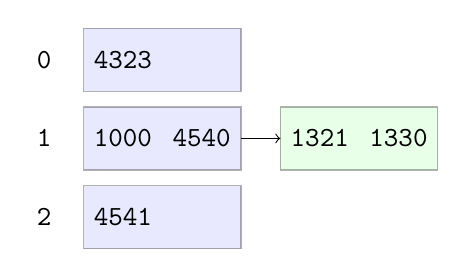
\begin{tikzpicture}
            \foreach \i in {0, 1, 2} {
                \node at (0, 3-\i) {\texttt{\i}};
                
                \draw[fill=blue!30, opacity=0.3] (0.5, \i+1.4) -- (0.5, \i+0.6) -- (2.5, \i+0.6) -- (2.5, \i+1.4) -- cycle;
            };
            \draw[fill=green!30, opacity=0.3] (3, 2.4) -- (3, 1.6) -- (5, 1.6) -- (5, 2.4) -- cycle;
            
            \node at (1, 1) {\texttt{4541}};
            \node at (1, 2) {\texttt{1000}};
            \node at (2, 2) {\texttt{4540}};
            \node at (1, 3) {\texttt{4323}};
            \node at (3.5, 2) {\texttt{1321}};
            \node at (4.5, 2) {\texttt{1330}};
            
            \draw[->] (2.5, 2) -- (3, 2);
        \end{tikzpicture}
    \end{figure}    
\end{example}
\begin{answer}
    \begin{itemize}
        \item First, we consider the hash file representation. We assume that each bucket has equal probability. 
        \begin{itemize}
            \item If the hashed value is 0, then we need to access 1 block in both the best, the average and the worst case.
            \item If the hashed value is 1, then we need to access 2 blocks in the worst case and 1 block in the worst case. In the average case, the number of block accesses is
            \[\frac{1 + 2}{2} = 1.5\]
            \item If the hashed value is 2, then we need to access 1 block in both the best, the average and the worst case.
        \end{itemize}
        So, the expected block access in the worst case is
        \[\frac{1}{3} \cdot 1 + \frac{1}{3} \cdot 2 + \frac{1}{3} \cdot 1 = \frac{4}{3}.\]
        In the best case, the expected block access is
        \[\frac{1}{3} \cdot 1 + \frac{1}{3} \cdot 1 + \frac{1}{3} \cdot 1 = 1.\]
        The expected block access in the average case is
        \[\frac{1}{3} \cdot 1 + \frac{1}{3} \cdot 1.5 + \frac{1}{3} \cdot 1 = 1.17\]
        block accesses. 
        
        \item If we use the heap file structure, we need 3 blocks to store the 6 tuples. So, in the worst case, we have 3 block accesses. In the best case, we just need 1 block access. The expected block access for heap representation in the average case is
        \[\frac{1 + 3}{2} = 2\]
        block accesses. 
        
        \item In the sequential file structure, we also have 3 blocks. In the average and the worst case, we have 
        \[\log_2 3 \approx 1.58\]
        block accesses. In the best case, we just need 1 block access. 
    \end{itemize}
\end{answer}

\begin{example}
    Assume that we have hash, heap and sorted file where:
    \begin{itemize}
        \item we have 3 blocks in heap and sorted file;
        \item we have 4 blocks in the hash file- 3 main blocks and 1 overflown block.
    \end{itemize}
    Also, let $k$ be the hash attribute, and let $p\%$ be the proportion of the queries that involve the attribute $k$. Find the best data structure (in the worst case) to store the values with respect to the ratio $p$.
\end{example}
\begin{answer}
    \begin{itemize}
        \item If the file is a heap we would need 3 block accesses in the worst case. The attribute $k$ does not matter because the search is always linear. 
        
        \item Next, assume that the file is sorted with respect to $k$. If the search uses the attribute $k$, then we can use a binary search algorithm to get the result in $O(\log_2 b)$ block accesses. Instead, if it does not use the attribute $k$, then we have to use the linear search in $O(b)$ block accesses. So, the expected number of block accesses in the worst case is
        \[p \cdot (\log_2 3) + (1 - p) \cdot 3 = 3 + p \cdot (\log_2 3 - 3).\]
        
        \item Now, if we use hash representation, we have
        \[p \cdot (\tfrac{1}{3} \cdot 1 + \tfrac{1}{3} \cdot 2 + \tfrac{1}{3} \cdot 1) + (1 - p) \cdot 3 = 4 - \tfrac{8}{3} p\]
        block accesses in the worst case.
    \end{itemize}
    We can plot these lines and see which option is better depending on the value of $p$.
    \begin{figure}[H]
        \centering
        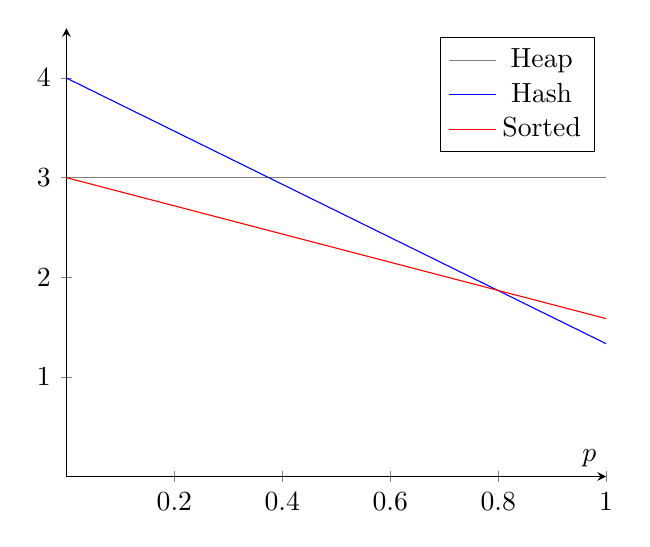
\begin{tikzpicture}
            \begin{axis}[
                axis lines=center,
                xlabel=$p$,
                xmin=0, ymin=0, ymax=4.5,
            ]
                \addplot[
                    domain=0:1,
                    samples=100,
                    gray
                ] {3};
                \addplot[
                    domain=0:1,
                    samples=100,
                    blue
                ] {4 - 8/3*x};
                \addplot[
                    domain=0:1,
                    samples=100,
                    red
                ] {3 + (ln(3)/ln(2) - 3)*x};
                \legend{Heap, Hash, Sorted}
            \end{axis}
        \end{tikzpicture}
    \end{figure}
    \noindent So, if $p < 0.8$, we should use the sorted representation. Instead, if $p > 0.8$, we should use the hash representation.
\end{answer}
\newpage

\section{Indexing Methodology}
\begin{example}
    Assume we have the \texttt{EMPLOYEE} table with key attribute \texttt{SSN}.
    \begin{itemize}
        \item We have $r = 300 \ 000$ records.
        \item A record takes $R = 100$ bytes.
        \item The block size is $B = 4 \ 096$ bytes.
        \item The attribute \texttt{SSN} occupies 9 bytes.
        \item A pointer occupies 6 bytes.
        \item The data files are sorted with respect to \texttt{SSN}.
    \end{itemize}
    We want to execute the query.
\begin{lstlisting}[language=SQL]
SELECT  *
FROM    EMPLOYEE
WHERE   SSN = k;
\end{lstlisting}
    Compute the number of block accesses we need to execute this query using a linear search, binary search and a primary index.
\end{example}
\begin{answer}
    The blocking factor is
    \[\textit{bfr} = \operatorname{floor}(B/R) = \operatorname{floor}(4096/100) = 40.\]
    So, the number of data blocks we need is
    \[b = \operatorname{ceil}(r/\textit{bfr}) = 7500.\]
    \begin{itemize}
        \item A linear search takes on average
        \[b/2 = 3750\]
        block accesses.
        
        \item A binary search takes on average
        \[\log_2 b \approx 11.9\]
        block accesses.
        
        \item The index entry has components: $\texttt{(SSN, Pointer)}$. We know that we need 9 bytes for SSN and 6 for the pointer, so we need 15 bytes for each index. Therefore, the indexing blocking factor is
        \[\textit{ibfr} = \operatorname{floor}(4096/15) = 273.\]
        We have 7 500 data blocks, so 7 500 index tuples. So, we need
        \[\textit{ib} = \operatorname{ceil}(7500/273) = 28\]
        blocks to store all the index files.
        
        Next, we compute the number of block accesses with the primary index. 
        \begin{itemize}
            \item We first search for the SSN in the index. Since the primary index is sorted with respect to the index, it takes about
            \[\log_2 28 \approx 4.8\]
            block accesses to find it. 
            \item After finding the index block, we need to load the data block. This takes 1 block access.
        \end{itemize}
        So, we have 5.8 block accesses to find the relevant tuple.
    \end{itemize}
\end{answer}

\begin{example}
    Assume we have the \texttt{EMPLOYEE} table with non-key attribute \texttt{DNO}.
    \begin{itemize}
        \item We have $r = 300 \ 000$ records.
        \item A record takes $R = 100$ bytes.
        \item The block size is $B = 4 \ 096$ bytes.
        \item The attribute \texttt{DNO} occupies 9 bytes.
        \item A pointer occupies 6 bytes.
        \item The data files are sorted with respect to \texttt{DNO}.
        \item There are 10 departments.
        \item The \texttt{DNO} values are uniformly distributed over the tuples, i.e. there are $30 \ 000$ employees in each department.
    \end{itemize}
    We want to execute the query
\begin{lstlisting}[language=SQL]
SELECT  *
FROM    EMPLOYEE
WHERE   DNO = x;
\end{lstlisting}
    Compute the number of block accesses we need to execute this query using a linear search and a clustering index.
\end{example}
\begin{answer}
    The blocking factor is
    \[\textit{bfr} = \operatorname{floor}(4096/100) = 40.\]    
    So, the number of blocks we need is
    \[b = \operatorname{ceil}(r/\textit{bfr}) = 7 \ 500.\]
    
    \begin{itemize}
        \item We first consider a linear scan with an exiting feature- we stop as soon as we have found all the tuples. Based on the uniformity assumption, each department has 750 blocks. If we have \texttt{DNO = 1}, then we retrieve the first 750 blocks and then stop. If \texttt{DNO = 2}, then we retrieve the first two 750 blocks and then stop. Assuming that it is equally likely for the \texttt{DNO} to take all these values and that the value \texttt{x} is a valid \texttt{DNO}, the expected block accesses is:
        \[\frac{1}{10} \cdot 750 + \frac{1}{10} (750 \cdot 2) + \dots + \frac{1}{10} (750 \cdot 10) = 4125.\]    
        
        \item Next, we consider a clustering index on DNO. The indexing blocking factor is
        \[\textit{ibfr} = \operatorname{floor}(4096/15) = 273.\]
        We have 10 data blocks, so we need
        \[\textit{ib} = \operatorname{ceil}(10/273) = 1\]
        block to store all the index files. When executing the query, we find the block pointer corresponding to \texttt{DNO = x} in 1 block access. Then, we load the 750 contiguous blocks to find all the relevant tuples. This requires 751 block accesses.
    \end{itemize}
\end{answer}


% In general, if we have $n$ clusters and $b$ blocks, then linear search with an exiting feature on an ordered data file is
% \[\frac{b(n+1)}{2n}.\]

% We should create a clustering index if it allows us to find the result in fewer block accesses. In particular, if we have $m$ clustering index blocks, $b$ data blocks and $n$ clusters, we should create the index if
% \[\log_2 m <  \frac{b(n-1)}{2n} \implies m < 2^{\frac{b(n-1)}{2n}.}\]
% Moreover, as $n \to \infty$, the linear search over an ordering non-key field with exiting feature is bound by $b/2$. So, as 
% i.e. we have an infinite number of distinct values, then the linear search over an ordering non-key field with exiting feature is bound by $b/2$, which is half of the naive linear search, i.e.
% \[\lim_{n \to \infty} \frac{b(n+1)}{2n} = \frac{b}{2} < b.\]

\begin{example}
    Assume we have the \texttt{EMPLOYEE} table with non-ordering key attribute \texttt{SSN}. 
    \begin{itemize}
        \item We have $r = 300 \ 000$ records.
        \item A record takes $R = 100$ bytes.
        \item The block size is $B = 4 \ 096$ bytes.
        \item The attribute \texttt{SSN} occupies 9 bytes.
        \item A pointer occupies 6 bytes.
    \end{itemize}
    We want to run the query
\begin{lstlisting}[language=SQL]
SELECT  *
FROM    EMPLOYEE
WHERE   SSN = x;
\end{lstlisting}
    Compute the number of block accesses we need using a linear scan and a secondary index on a non-ordering key attribute \texttt{SSN}.
\end{example}
\begin{answer}
    The blocking factor is
    \[\textit{bfr} = \operatorname{floor}(B/R) = 40\]
    records per block. So, we need
    \[b = \operatorname{ceil}(r/\textit{bfr}) = 7500\]
    blocks to store all the data.
    \begin{itemize}
        \item First, we consider a linear search. Since the attribute \texttt{SSN} is key, this would take on average 
        \[b/2 = 3750\]
        block accesses.

        \item Next, we consider using the secondary index. An index entry takes 15 bytes. So, the index blocking factor is
        \[\textit{ibfr} = \operatorname{floor}(4096/15) = 273.\]
        Since we are using a dense index, we have 300 000 index entries. So, we need
        \[\textit{ib} = \operatorname{ceil}(300 \ 000/273) = 1099\]
        blocks. 
    
        To search for a single employee, we first search within the index. Since the index file is sorted, we can find it in
        \[\log_2(\textit{ib}) \approx 10.1\]
        block accesses. Next, we load the unique block pointed by the index entry. So, we require $11.1$ block accesses to find the relevant tuple.
    \end{itemize}
\end{answer}

% \begin{example}
%     Assume we have the \texttt{EMPLOYEE} table with non-ordering, non-key attribute \texttt{DNO}, where 
%     \begin{itemize}
%         \item we have $r = 300 \ 000$ records.
%         \item a record takes $R = 100$ bytes.
%         \item the block size is $B = 4 \ 096$ bytes.
%         \item the attribute \texttt{DNO} occupies 9 bytes.
%         \item a pointer occupies 6 bytes.
%         \item there are 4 blocks of pointers satisfying \texttt{DNO = 3}.
%     \end{itemize}
%     We want to execute the query.
% \begin{lstlisting}[language=SQL]
% SELECT  *
% FROM    EMPLOYEE
% WHERE   DNO = 3;
% \end{lstlisting}
%     Compute the number of block accesses we need using a secondary indexing on \texttt{DNO}.
% \end{example}
% \begin{answer}
%     We can use binary search in level 2. There is only one block at level 1 corresponding to \texttt{DNO = 3}, so we can use that to load all the 4 blocks that have \texttt{DNO = 3}. 
    
%     If we do not have this index, we need to linearly scan all the blocks since it is not a unique value. So, we need to access all 7500 blocks.
% \end{answer}

\begin{example}
    Now, assume that we have the \texttt{EMPLOYEE} table on the non-ordering key attribute \texttt{SSN}. 
    \begin{itemize}
        \item We have $r = 300 \ 000$ records.
        \item A record takes $R = 100$ bytes.
        \item The block size is $B = 4 \ 096$ bytes.
        \item The attribute \texttt{SSN} occupies 9 bytes.
        \item A pointer occupies 6 bytes.
    \end{itemize}
    What level of multilevel index should we build? Use this value to predict the number of block accesses when using the index to find a tuple given the \texttt{SSN} value.
\end{example}
\begin{answer}
    The blocking factor is
    \[\textit{bfr} = \operatorname{floor}(B/R) = 40\]
    records per block. So, we need
    \[b = \operatorname{ceil}(r/\textit{bfr}) = 7500\]
    blocks to store all the data.

    An index entry has tuples with attributes \texttt{SSN} and a pointer. So, this takes 15 bytes. In that case, the index blocking factor is
    \[m = \operatorname{floor}(4096/15) = 273.\]
    Therefore, at L1 index, we have 
    \[b_1 = \operatorname{ceil}(300 \ 000/m) = 1099\]
    index blocks, since the index is dense. So, at L2, we have $1 \ 099$ index entries, and we require
    \[b_2 = \operatorname{ceil}(b_1/m) = 5\]
    blocks to store them. Furthermore, at level-3, we have $5$ index entries, and we just require
    \[b_3 = \operatorname{ceil}(b_2/m) = 1\]
    block for it. Since we just need 1 block here, we build a 3-level index. 
    
    Now, to find the unique employee we are searching for, we just need 4 block accesses- 3 going from one index level to a lower level, and the last one to get the data block.
\end{answer}
\newpage

\section{B and B+ Trees}
\begin{example}
  Assume that we have created a 3-level B tree of order $p = 23$ that is $69\%$ full.  Compute the number of data and tree pointers we can store in the tree. Moreover, assume the following.
  \begin{itemize}
      \item The block size is $B = 512$ bytes.
      \item A data pointer takes $Q = 7$ bytes.
      \item A tree pointer takes $P = 6$ bytes.
      \item A key value takes $V = 9$ bytes.   
  \end{itemize}
  Using this information, compute the number of blocks we have in total.
\end{example}
\begin{answer}
    In each block, we store
    \[69\% \times 23 \approx 16\]
    tree pointers, and 15 data pointers. In that case, the root block contains 16 tree pointers and 15 data pointers. At level 1, we have 16 blocks, each of which contains 16 tree pointers and 15 data pointers. At level 2, we have $16^2$ blocks, each of which contains 16 tree pointers and 15 data pointers. At level 3, we have $16^3$ blocks, each of which contains no tree pointers and 15 data pointers. This is summarised in the table below.
    \begin{table}[H]
        \centering
        \begin{tabular}{|c|c|c|}
            \hline
            level & data pointers & tree pointers \\
            \hline
            0 & 15 & 16 \\
            1 & $16 \cdot 15$ & $16^2$ \\
            2 & $16^2 \cdot 15$ & $16^3$ \\
            3 & $16^3 \cdot 15$ & 0 \\
            \hline
        \end{tabular}
    \end{table}
    In total, we can store 
    \[15 + 16 \cdot 15 + 16^2 \cdot 15 + 16^3 \cdot 15 = 65 \ 535\]
    data pointers and 
    \[16 + 16^2 + 16^3 = 4368\]
    tree pointers. 
    % If we want to add an extra tuple, then we would need to add another level. Since B trees are balanced, we need to add all $16^4$ tree pointers. But then, 93.3\% of the leaf nodes at level 4 are empty. We need to choose a good value for $p$ to reduce this redundancy. This gives rise to another challenge.    

    % In that case, an B+ Tree node takes
    % \[65 \ 536 \cdot (7 + 9) + 4 \ 368 \cdot 6 = 1.02 \text{ MB}.\]
    A block has size
    \[15 \cdot (7 + 9) + 16 \cdot 6 = 336 \text{ bytes}.\]
    So, the blocking factor 
    \[\textit{bfr} = \operatorname{floor}(512/336) = 1.\]
    In that case, we need 
    \[1 + 16 + 16^2 + 16^3 = 4369\]
    blocks to store the 3-level B tree.
\end{answer}

\begin{example}
    Assume we have the following query.
\begin{lstlisting}[language=SQL]
SELECT  * 
FROM    EMPLOYEE
WHERE   SSN >= 3 AND SSN <= 10;
\end{lstlisting}    
    We are also given the following B and B+ Trees.
    \begin{figure}[H]
        \centering
        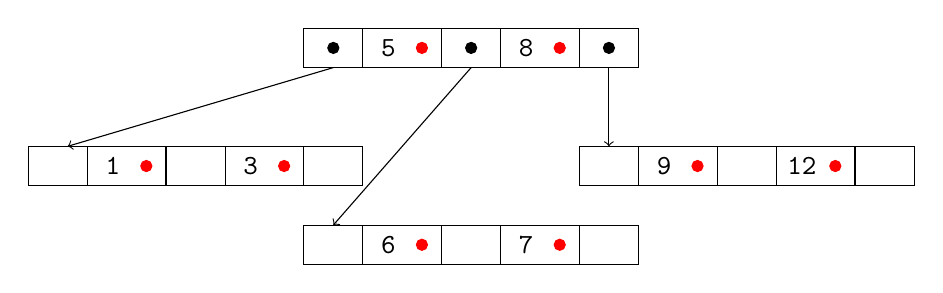
\begin{tikzpicture}
            \bnode{0}{0}{5, 8} 
            \bnodeend{-3.5}{-1.5}{1, 3} 
            \bnodeend{0}{-2.5}{6, 7} 
            \bnodeend{3.5}{-1.5}{9, 12} 
            
            \draw[->] (0.375, 0) -- (-3, -1);
            \draw[->] (2.125, 0) -- (0.375, -2);
            \draw[->] (3.875, 0) -- (3.875, -1);
        \end{tikzpicture}
    \end{figure}
    \begin{figure}[H]
        \centering
        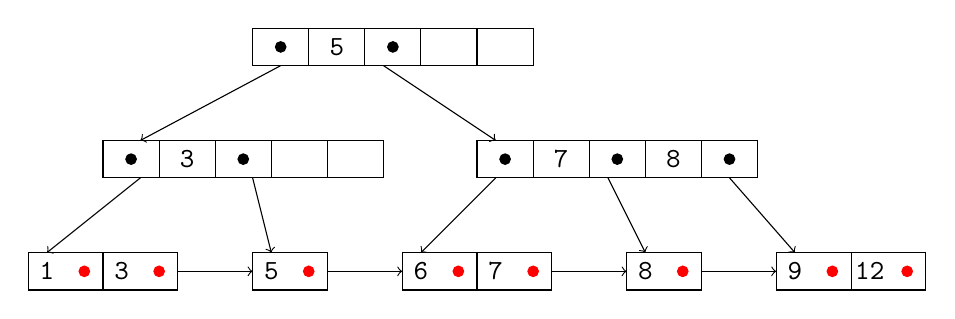
\begin{tikzpicture}[scale=0.95]
            \bplusinternalnodesng{0}{0}{5}
            \bplusinternalnodesng{-2}{-1.5}{3}
            \bplusinternalnodedbl{3}{-1.5}{7, 8}
            \bplusleafnodedbl{-3}{-3}{1, 3}
            \bplusleafnodesng{0}{-3}{5}
            \bplusleafnodedbl{2}{-3}{6, 7}
            \bplusleafnodesng{5}{-3}{8}
            \bplusleafnodedbl{7}{-3}{9, 12}

            \draw[->] (0.375, 0) -- (-1.5, -1);
            \draw[->] (1.75, 0) -- (3.25, -1);

            \draw[->] (-1.5, -1.5) -- (-2.75, -2.5);
            \draw[->] (0, -1.5) -- (0.25, -2.5);
            \draw[->] (3.25, -1.5) -- (2.25, -2.5);
            \draw[->] (4.75, -1.5) -- (5.25, -2.5);
            \draw[->] (6.375, -1.5) -- (7.25, -2.5);
            
            \draw[->] (-1, -2.75) -- (0, -2.75);
            \draw[->] (1, -2.75) -- (2, -2.75);
            \draw[->] (4, -2.75) -- (5, -2.75);
            \draw[->] (6, -2.75) -- (7, -2.75);
        \end{tikzpicture}
    \end{figure}
    Compute the number of block accesses we need in order to execute this query for both a B Tree and a B+ Tree.
\end{example}
\begin{answer}
    \begin{itemize}
        \item First, we use the B Tree. We access the root block and get the values \texttt{SSN = 5} and \texttt{SSN = 8}. Since they are both in the range, we need to access all the 3 branches. 
        
        So, we need 4 block accesses within the B Tree, and 6 data block accesses.

        \item Next, we use the B+ Tree. We access the root block and get the value \texttt{SSN = 5}. We want to find the tuple satisfying \texttt{SSN = 3}, so we just need to take the left branch. Now, we take the left branch in level 1. Then, we have found the first block that we require. We can make use of the sorted structure of the leaf nodes to find all the other tuples that satisfy the given condition. 
        
        So, we need 2 block accesses within the internal nodes of the B+ Tree, 5 block accesses within the leaf nodes of the B+ Tree, and 6 data block accesses.
    \end{itemize}    
\end{answer}

% By removing the data pointers from internal nodes, we obtain higher fan out, thus more index entries and quicker search process. We show this with an example. Assume we have block size $B = 512$ bytes, key value $V = 9$ bytes, data pointer $Q = 7$ bytes, tree pointer $P = 6$ bytes. A B tree node will take up
% \[p \cdot 6 + (p-1) \cdot (9+7) = 22p - 16\]
% bytes. The biggest possible value of $p$ satisfying $22p - 16 \leq 512$ is $p = 24$. On the other hand, for a B+ tree internal node, we require
% \[p \cdot 6 + (p-1) \cdot 9 = 15p - 9\]
% bytes. Here, the biggest possible value of $p$ is $p = 34$. For a B+ leaf node, we require
% \[p_L \cdot (9 + 7) + 9\]
% bytes. So, the biggest possible value of $p_L$ is $p_L = 31$. Clearly, we can store more entries in both the B+ tree nodes compared to a B tree. The fan out has indeed increased.

\begin{example}
    Construct a 3-level B+ Tree of order $p = 34$ and $p_L = 31$ that is $69\%$ full. Also, compute the number of blocks we have in total.
\end{example}
\begin{answer}
    We can fit 
    \[69\% \times 34 = 23\]
    tree pointers in an internal node and 
    \[69\% \times 31 = 21\]
    data pointers in a leaf node. The table below summarises the number of tree pointers and key values we can hold in the first 2 levels.
    \begin{table}[H]
        \centering
        \begin{tabular}{|c|c|c|}
            \hline
            level & key values & tree pointers \\
            \hline
            0 & 22 & 23 \\
            1 & $23 \cdot 22$ & $23^2$ \\
            2 & $23^2 \cdot 22$ & $23^3$ \\
            \hline
        \end{tabular}
    \end{table}
    \noindent So, we can fit 12 720 tree pointers. At level 3, we can fit $23^3 \cdot 21 = 255 \ 507$ key values and data pointers. Assuming that one B+ block fits one node, we require
    \[1 + 23 + 23^2 + 23^3 = 12 \ 720\]
    blocks.
\end{answer}

\begin{example}
    % Next, we compare block accesses and the number of extra blocks required to evaluate a query based on a secondary, non-ordering key field, where:
    Assume that we are given the following query.
\begin{lstlisting}[language=SQL]
SELECT  *
FROM    EMPLOYEE
WHERE   SSN = k;
\end{lstlisting}
    We are told the following:
    \begin{itemize}
        \item the size of a block $B = 512$ bytes;
        \item the number of tuples $r = 100 \ 000$;
        \item the blocking factor $\textit{bfr} = 10$ records/block;
        \item a pointer takes up 10 bytes;
        \item the indexing key takes 10 bytes.
    \end{itemize}
    Moreover, we have the following primary access paths:
    \begin{itemize}
        \item A secondary index over \texttt{SSN}.
        \item A B+ tree of order 25 over \texttt{SSN}.
    \end{itemize}
    Compute the number of block accesses we require to execute the query using a linear search, secondary index and the B+ Tree.
\end{example}
\begin{answer}
    \begin{itemize}
        \item First, we consider a linear search. Since there are 100 000 records and $\textit{bfr} = 10$, we have 10 000 data blocks. On average, the linear search will require 5000 block accesses since \texttt{SSN} is a key attribute.
        
        \item Next, we consider a secondary index. Since the index is secondary, we need a dense index- every data record appears in the index, with a data pointer (10 bytes) and the key value (10 bytes). So, each record takes up 20 bytes. We know a block can store 512 bytes, so each block can hold
        \[\operatorname{floor}(512/20) = 25\]
        tuples. In that case, we require
        \[\operatorname{ceil}(100 \ 000/25) = 4 \ 000\]
        extra blocks to store the secondary index. Moreover, using the secondary index, we require 
        \[\log_2 4000 \approx 12\]
        block accesses to find the right tuple on the secondary index file, and then a further data block access to retrieve the tuple. In total, the search requires 13 block accesses.
        
        \item Finally, we consider a B+ tree index of order 25. Assuming the nodes are completely full, each internal node can hold 24 key values and 25 tree pointers, and a leaf block can hold 24 key values and data pointers. A pointer and an indexing key take 10 bytes, so an internal node takes up
        \[25 \cdot 10 + 24 \cdot 10 = 490\]
        bytes. Moreover, a leaf node takes up
        \[24 \cdot 10 + 24 \cdot 10 + 10 = 490\]
        bytes. So, we can fit 1 internal/leaf node per block. Next, we compute the level of B+ Tree we need to store the $100 \ 000$ tuples:
        \begin{table}[H]
            \centering
            \begin{tabular}{|c|c|c|}
                \hline
                level & key values & tree pointers \\
                \hline
                0 & 24 & 25 \\
                1 & $25 \cdot 24$ & $25^2$ \\
                2 & $25^2 \cdot 24$ & $25^3$ \\
                \hline
            \end{tabular}
        \end{table}
        So, at level 3, we have
        \[25^3 \cdot 24 = 375 \ 000\]
        data pointers/key values. Since we only have $100 \ 000$ tuples, we are only using up about $30\%$ of the leaf nodes. Moreover, we need
        \[1 + 25 + 25^2 + 25^3 = 16 \ 276\]
        extra blocks to store the B+ tree. 
        
        Nonetheless, we can find a tuple using a B+ tree with just 5 block accesses:
        \begin{enumerate}
            \item we access the root internal node, 
            \item we descend to the relevant level 1 internal node,
            \item we descend to the relevant level 2 internal node,
            \item we descend to the relevant level 3 leaf node, and
            \item we retrieve the relevant data block.
        \end{enumerate}
    \end{itemize}
\end{answer}

\begin{example}
    Assume that we have the query
\begin{lstlisting}[language=SQL]
SELECT  AVG(SALARY) 
FROM    EMPLOYEE 
WHERE   SSN >= L AND SSN <= U;
\end{lstlisting}
    Here,
    \begin{itemize}
        \item there are $b = 1 \ 250$ blocks,
        \item there are $n = 1 \ 250$ employees,
        \item the blocking factor $\textit{bfr} = 1$ employee/block,
        \item \texttt{SSN} takes up 10 bytes,
        \item a pointer takes up $P = 10$ bytes,
        \item the B+ tree is of order $p = 5$ and $p_L = 10$,
        \item the leaf nodes are full,
        \item the SSN values range from 1 to 1250.
    \end{itemize}    
    Find the maximum ratio
    \[\alpha = \frac{U - L}{1250}\] 
    of \texttt{SSN} values selected by the query such that searching using the B+ Tree is more efficient than a linear scan.
\end{example}
\begin{answer}
    We know that an internal node can hold 4 key values and 5 data pointers. So, we need a 3-level B+ tree so that the leaf nodes can hold the $1 \ 250$ records. The table below shows how many entries are present in the internal nodes.
    \begin{table}[H]
        \centering
        \begin{tabular}{|c|c|c|}
            \hline
            level & key values & tree pointers \\
            \hline
            0 & 4 & 5 \\
            1 & $5 \cdot 4$ & $5^2$ \\
            2 & $5^2 \cdot 4$ & $5^3$ \\
            \hline
        \end{tabular}
    \end{table}
    \noindent So, at level 3, we precisely have
    \[5^3 \cdot 10 = 1 \ 250\]
    key values/data pointers. 
    
    When we execute this range query over the B+ tree, we need 3 block accesses to descend from the root to the leaf node containing the data pointer for \texttt{SSN = L}. Each leaf node contains 10 blocks, so we approximately need to access 
    \[\frac{U - L}{10} = \frac{1250 \alpha}{10} = 125 \alpha\]
    leaf blocks. Moreover, we need to access all $U - L = 1250 \alpha$ data blocks. Overall, we need to access
    \[3 + 125 \alpha + 1250 \alpha = 3 + 1375 \alpha\]
    blocks. 
    
    Using a linear search, we need to access all the 1250 blocks since the tuples are not sorted with respect to \texttt{SSN}. Therefore, for B+ trees to be useful, we require 
    \[3 + 1375 \alpha < 1250 \implies \alpha < \frac{1247}{1375} \approx 0.906.\]
    So, if the ratio is less than $90.6\%$, then we should use B+ tree. Otherwise, we should use linear searching.
\end{answer}

\end{document}
